\documentclass{article}
\usepackage{graphicx} % Required for inserting images
\usepackage{amsmath}
\usepackage{amssymb}
\usepackage[a4paper, total={7.5in, 10.85in}]{geometry}

\title{A Different Way of Thinking About The Coin Rotation Paradox}
\author{Lily Sun (Guest Writer)}
\date{}

%% \blurb{In 1982, there was a problem on the SAT that was so difficult that none of the test takers were able to correctly solve it. Well, perhaps that's not entirely true, as none of the five choices on the multiple-choice question were correct. The problem came to be known as the Coin Rotation Paradox...}

\begin{document}

\maketitle
In 1982, there was a problem on the SAT that was so difficult that none of the test takers were able to correctly solve it. Well, perhaps that's not entirely true, as none of the five choices on the multiple-choice question were correct. The problem came to be known as the Coin Rotation Paradox. It is as follows:

"The radius of circle $A$ is $\frac{1}{3}$ of the radius of circle $B$. Circle $A$ rolls around circle $B$ one trip back to its starting point. How many times will circle $A$ revolve in total?"

\begin{center}
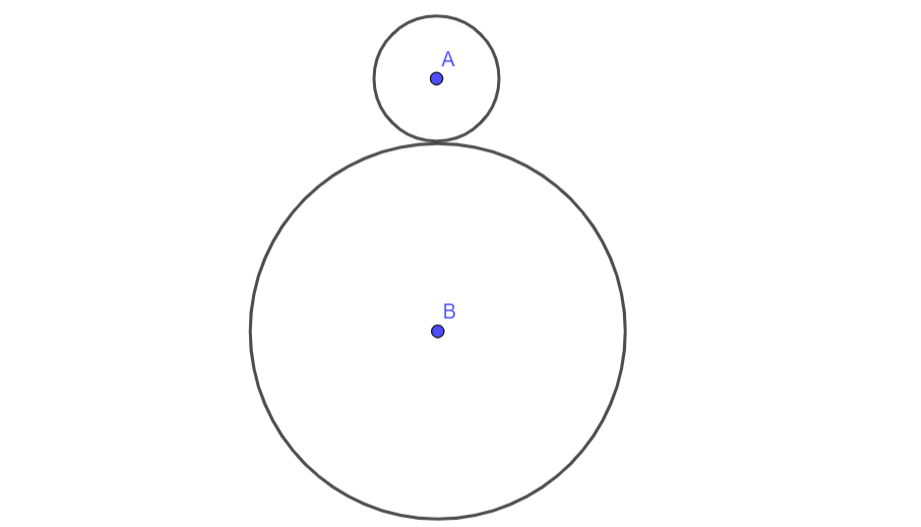
\includegraphics[scale=0.5]{images/circleAandcircleB.png}
\end{center}

It may be tempting to assume that the answer is $3$, as the circumference of circle $A$ is a third of the circumference of circle $B$, thus having to roll three times to cover the distance of the circumference of circle $B$. However, the real answer, $4$, is a bit counter-intuitive.

Let's take a step back and think about a simpler version of this problem: rotating a square $A$ of length $1$ around a congruent square, $B$. Take a moment to think about how many revolutions square $A$ will make before completing the rotation around square $B$.

\begin{center}
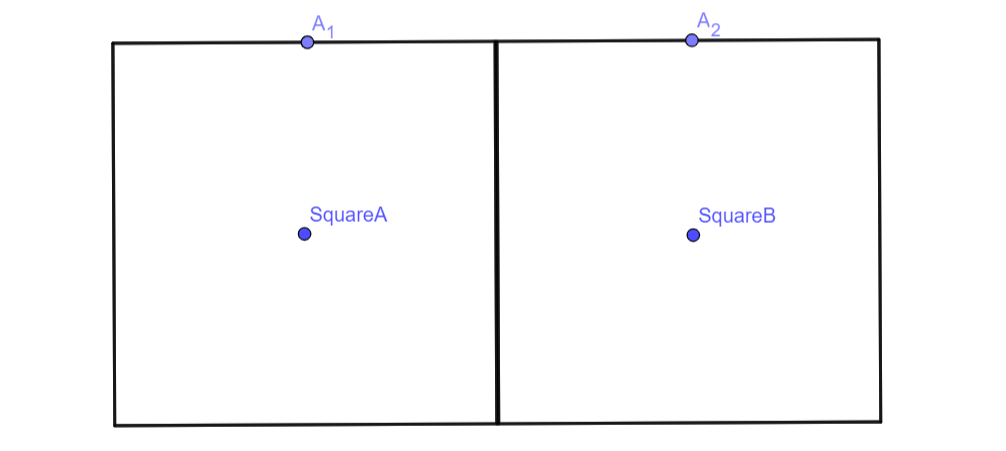
\includegraphics[scale=0.5, angle = -0.5]{images/squareAandsquareB.png}
\end{center}

For side $A_1$ to match up with $A_2$, square $A$ needs to turn exactly $180^{\circ}$. With two turns, the square has already traveled $360^{\circ}$, or an entire revolution! This means that for a square with side length $1$ to rotate around a congruent square, it will revolve twice ($720^{\circ}$), not once. This means that instead of looking at the distances, we should look at angles. To generalize this finding, what if we had two congruent n-gons? Each time n-gon $A$ rotates, it covers the angle that is explementary to the two interior angles of the n-gons. Let $n$ denote the number of sides in our arbitrary n-gon. This means that the interior angles of our n-gon is $\frac{180(n-2)}{n}$. Each time n-gon $A$ rotates, it will rotate $360 - 2 \cdot \frac{180(n-2)}{n}$ degrees, which can be simplified to $720^{\circ}$. Thus, for each n-gon, it will make two complete revolutions each time it rotates around a congruent n-gon. For our n-gon to be a circle, we have

$$\lim\limits_{n\to\infty}\ 360 - 2 \cdot \dfrac{180(n-2)}{n} = 720,$$

which means that a circle will always make two revolutions when rotating around a circle of the same radius. 

With this in mind, what happens when circle $A$ has a radius that is $\frac{1}{3}$ of the radius of circle $B$, instead of being congruent? We again simplify the problem such that we have a square of side length $1$ and a regular dodecagon also of side length $1$. 

\begin{center}
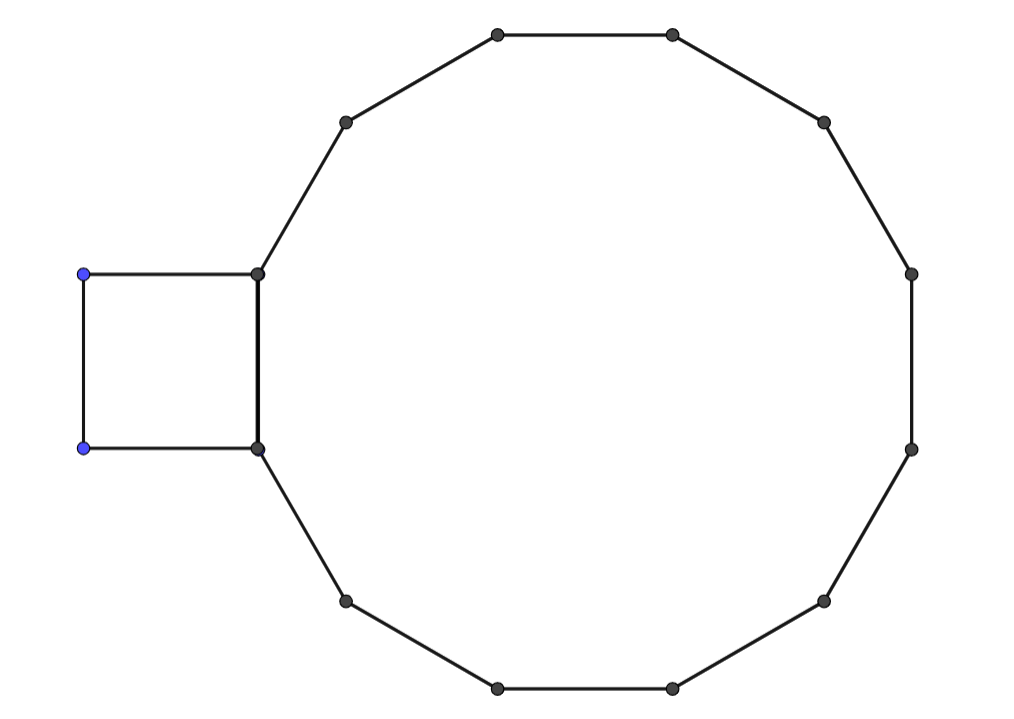
\includegraphics[scale=0.5]{images/squareanddodecagon.png}
\end{center}

The circumference of our square is $4$ and the circumference of the regular dodecagon is $12$, three times that of the square. How many revolutions will the square make around the dodecagon? Let's think about this without calculating the exact angles. If the square and the dodecagon were rotating at the same time (the dodecagon is rotating in the opposite direction of the square), the square would have made three revolutions once the dodecagon had made one, once the original sides met again. Because angles are the determining factor for the number of revolutions made, a revolution made by an n-gon with more sides is equivalent to a revolution made by an n-gon with less sides, because they both traveled $360^{\circ}$. This means that, if the dodecagon remained still, the square would undergo $3+1=4$ revolutions to travel around the dodecagon. Next, while keeping the circumference of the square and the dodecagon constant, we keep adding sides to the polygons until they become $\infty$-gons, or two circles. Adding sides won't change the number of revolutions the smaller polygon makes because the relative ratios of the two polygons remain the same: $1:3$. The circle that was once the square has a radius that is $\frac{1}{3}$ of the radius of the circle that was once the dodecagon,  matching the problem statement. Thus, the answer to the Coin Rotation Paradox is indeed $4$, not $3$.

\begin{center}
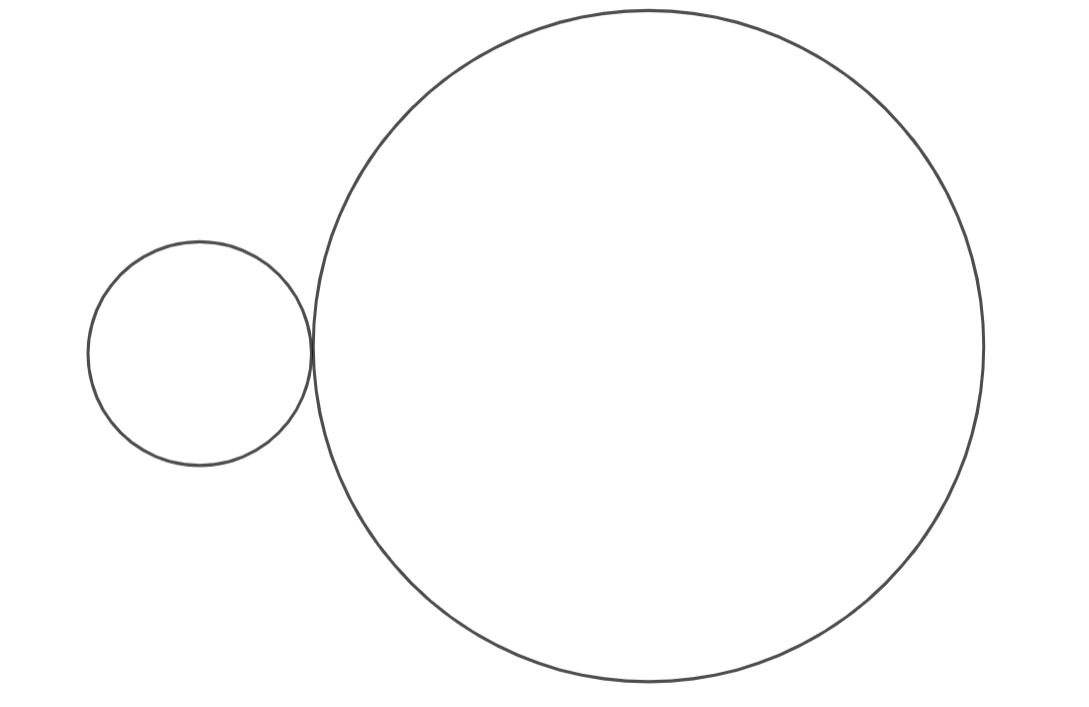
\includegraphics[scale=0.5]{images/weincreasethesidestoinfinity.png}
\end{center}

However, this begs the question: "Why are humans inclined to think that the answer is $3$?". If the problem had instead been that the bigger circle was rolled out into a string, to which the smaller circle traveled along that string, the answer would have indeed been $3$. However, that doesn't take into account the curvature of the bigger circle that the smaller circle has to travel around. But why the majority people attempting this problem didn't take that into account leaves us wondering: why does this problem seem to go against the majority of human intuition? 

\end{document}
